\chapter{Analyse}


\section{Domäne}

Die Applikation besitzt, wenn man die Daten selbst nicht miteinbezieht, ein relativ simples Domänen-Modell, wie in \cref{fig:pd:domain-model} zu sehen ist. Der Endbenutzer kann mehrere Dateien ablegen oder bereits vorhandene transformieren. Da das Resultat von Dateien oder Transformationen dasselbe ist, werden diese mit dem Oberbegriff Datenpaket\footnote{Im Frontend: ``Package''} versehen.

\begin{figure}[H]
    \centering
    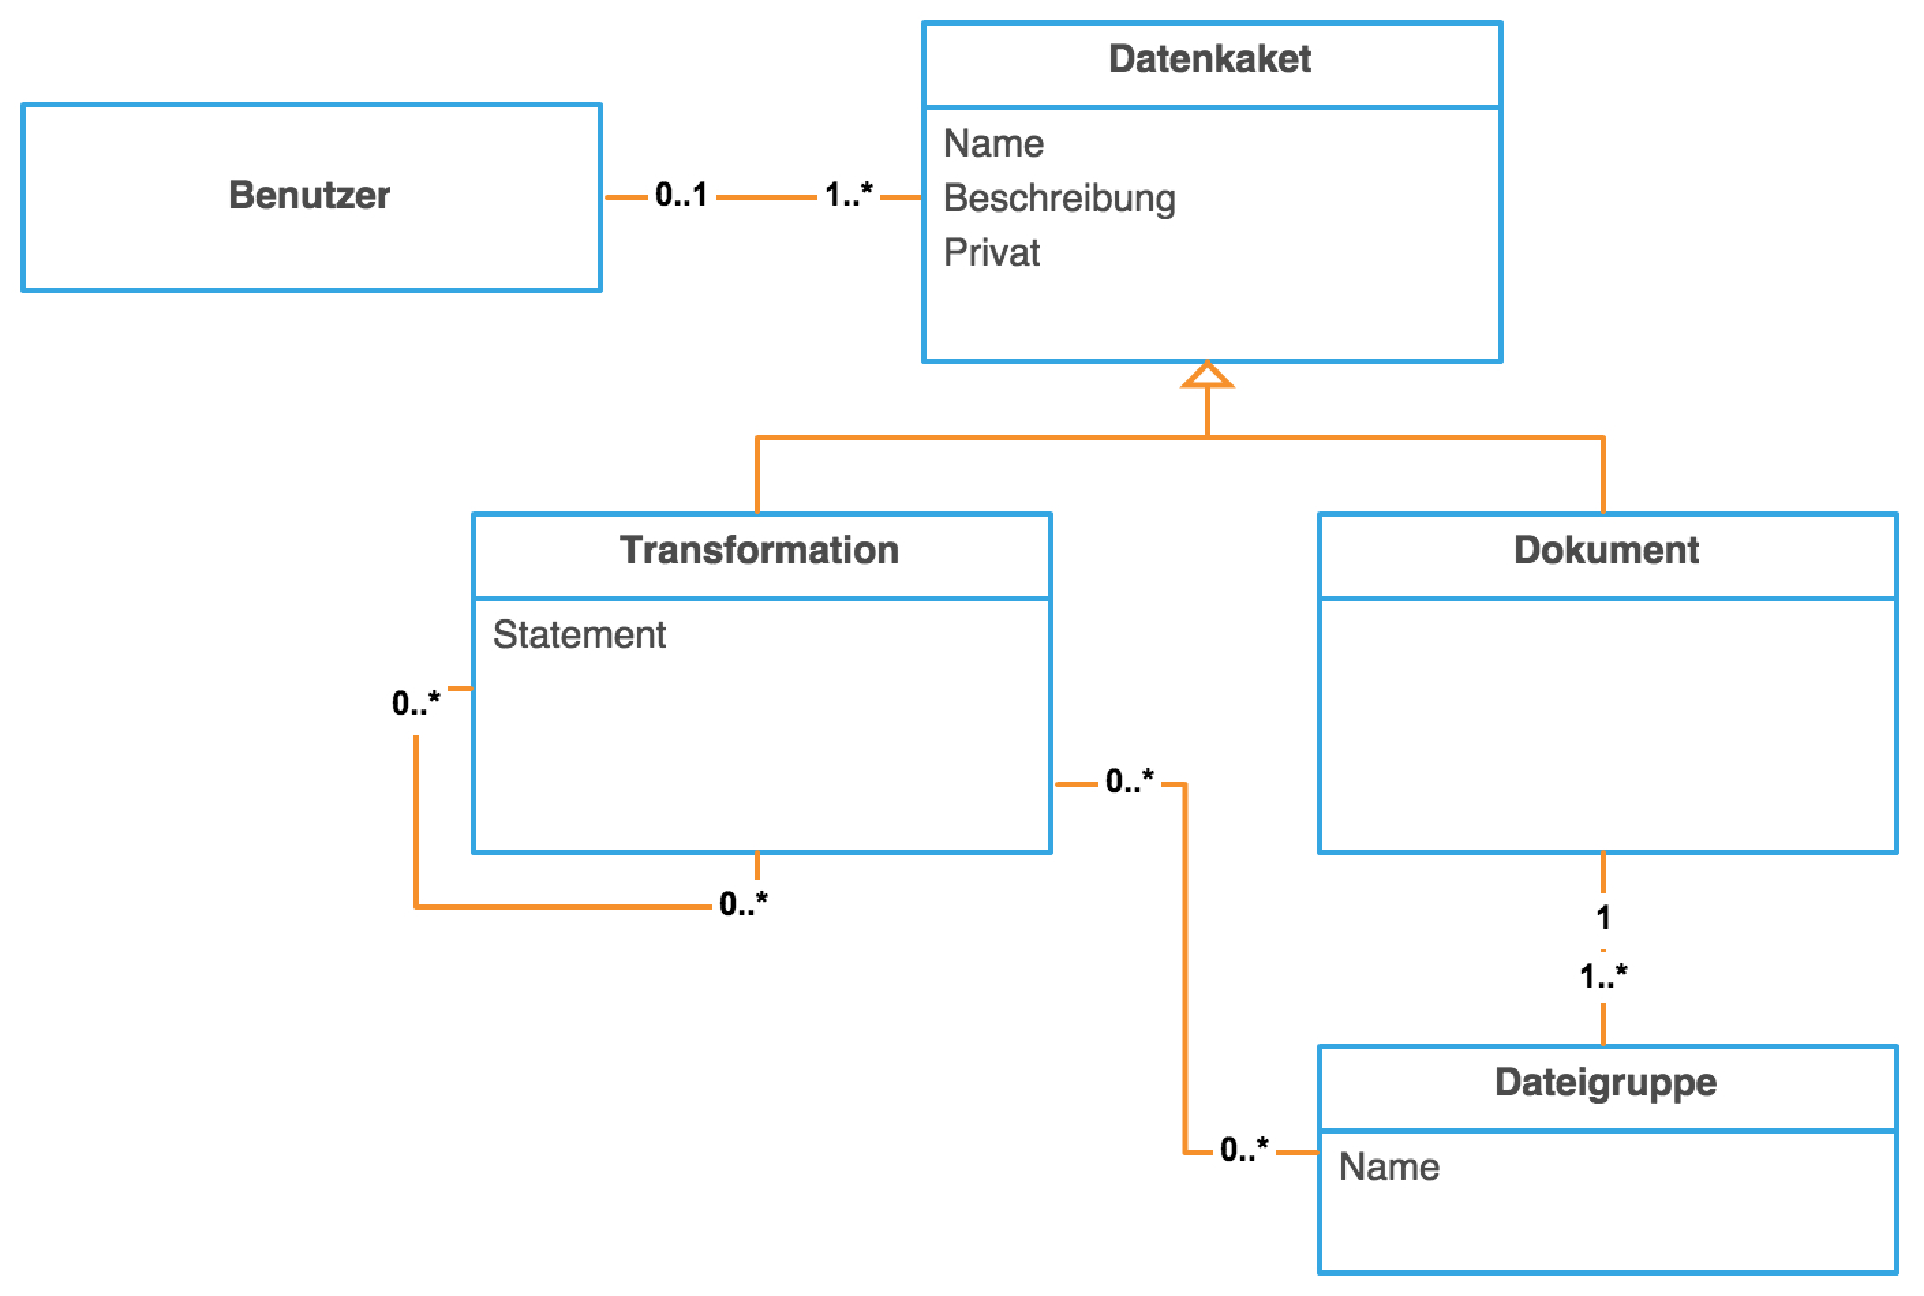
\includegraphics[width=0.8\linewidth]{fig/domain-model.pdf}
    \caption{Domäne OpenDataHub}
    \label{fig:pd:domain-model}
\end{figure}

\section{Dateiformate}

In diesem Abschnitt werden die durch den Kunden gewünschten oder zur Realisierung der Anwendungsfälle in \cref{sec:pd:usecases} benötigten Dateiformate und deren Eigenheiten beschrieben.

\subsection{CSV}
Das \acf{csv} gilt trotz vielen Schwächen als universelles Austausch/Exportformat für einfache Anwendungsfälle und sollte deshalb zwingend unterstützt werden. Eine \acs{csv} Datei enthält einen Datensatz pro Zeile und die Spalten üblicherweise durch Kommas oder Semikolon getrennt. Die erste Zeile enthält die Namen der einzelnen Felder.

\subsubsection{Erweiterung mit Typen und Geo-Daten}

\gls{geocsv} ist eine durch das Geometa-Lab der HSR spezifizierte Erweiterung der CSV Spezifikation um Geo-Daten mit folgenden Eigenheiten\cite{sfkeller,geocsv,gdal-csv}:

\begin{itemize}
\item Eine optionale Datei mit Endung \path{.csvt} spezifiziert auf einer einzigen Zeile die Datentypen genauer
\item Der spezielle Datentyp ``WKT'' für Geometrien im \gls{wkt} Format
\item Die speziellen Datentypen ``Point(x)'', ``Point(y)'' oder ``CoordX'' bzw. ``CoordY'' für den Spezialfall einer Punktgeometrie
\item Eine optionale Datei mit der Endung \path{.prj} zur Angabe des Referenzsystems, ebenfalls im \gls{wkt} Format\footnote{Achtung, das \path{.prf} Format von ESRI sieht sehr ähnlich aus, enthält jedoch weniger Informationen!}
\item Nur ein Geometrie-Objekt/Spalte pro Datei
\end{itemize}


\subsection{Excel}
Da viele nicht-technische Benutzer mit Microsoft Excel arbeiten\cite{sfkeller} oder Daten im Excel Format anliefern, müssen sowohl der alte Excel 2003 (xls) sowie der neue OpenXML (xlsx) Formate unterstützt werden.

\subsection{GeoJSON}
\gls{geojson} ist eine auf JSON basierende Schema-Spezifikation für Geo-Daten. Dieses Format ist heutzutage weit verbreitet und fast überall wo mit Geo-Daten hantiert wird unterstützt.

\subsection{GeoPackage}
GeoPackage ist ein relativ neues, auf SQLite basiertes, Format. Es ist sehr nahe an SpatiaLite, welches mit Version 4.2 auf GeoPackage wechselt.

\subsection{GML}
\gls{gml} ist ein auf XML basierendes Format für Geo-Daten und ist das Standard-Ausgabeformat von \acs{wfs}-Servern.


\subsection{INTERLIS}
\gls{interlis} besteht aus einer Modellbeschreibungssprache und einem Transferformat. Da es praktisch nur in der Schweiz zum Einsatz kommt ist die Unterstützung in kommerzieller Software mässig bis nicht vorhanden.

\gls{interlis} existiert in zwei Versionen: \gls{interlis} 1 verwendet ein zeilenbasiertes Transfer-Format, während für \gls{interlis} 2 XML gewählt wurde. Mit wenigen Ausnahmen stellt \gls{interlis} 2 eine Erweiterung von \gls{interlis} 1 um Objekt-orientierte Features dar.

\subsection{KML}
\gls{kml} ist wie \gls{gml} ebenfalls ein auf \acs{xml} basierendes Format, welches in Google Earth Verwendung findet. Speziell bei KML, ist dass es lediglich das Referenzsystem 4326 (klassisches lat/lon) unterstützt.


\subsection{ESRI Shapefile}
Das Shapefile ist ein von der Firma ESRI spezifiziertes Format zum Austausch von Geo-Daten. Es wird von fast allen Bibliotheken und Systemen unterstützt und eignet sich somit als universelles Austauschformat für Geo-Daten. Das Shapefile wird immer wieder aufgrund dessen Schwächen kritisiert. Da wären beispielsweise die Limitation der Spaltennamen auf 8 Zeichen sowie von Textspalten auf 255 Zeichen. Aus diesem Grund versuchen viele das veraltete Shapefile durch ein moderneres Format wie GeoJSON oder GeoPackage abzulösen \cite{sfkeller}.

\subsection{WFS}
Bei \gls{wfs} handelt es sich um einen speziellen Webservice für Geo-Daten. Die Daten können üblicherweise im \gls{gml} Format bezogen werden. Da es sich dabei um einen weit verbreiteten Standard des \gls{ogc} handelt, sollte die Applikation einen direkten Bezug von Daten via einem \acs{wfs} Server ermöglichen.

\subsection{XML}
Da es sich bei \acs{xml} um eine potenziell verschachtelte Datenstruktur handelt, wird vorerst nur eine flache Version ähnlich der von der API von \purl{http://truckinfo.ch} gelieferten in \cref{sec:pd:usecases} beschriebenen Daten. 

\subsection{JSON}
Auch bei JSON handelt es sich um ein Format mit Schachtelungsmöglichkeit. Aus diesem Grund wird auch hier vorerst nur die oberste Ebene betrachtet.


\section{Datenspeicherung}
Ein Ziel dieser Arbeit ist die Erstellung eines Datenhubs, welcher es Anbietern ermöglicht, ihre Daten anderen zur Verfügung zu stellen. 

Zur Speicherung der Daten stehen folgende Varianten zur Auswahl.

\subsection{File-basiert}
Die Daten werden direkt im Dateisystem gespeichert. Um Konflikte zwischen Dateinamen zu vermeiden muss ein Hashing-Schema definiert und verwendet werden. Metadaten zu den Dokumenten werden in einer Datenbank hinterlegt.

Die Daten werden in ihrem Ursprungsformat belassen, bis ein Nutzer eine Transformation auswählt und anwendet. Die Resultate einer solchen Transformation können direkt wieder im Dateisystem zwischengespeichert werden um weitere Abfragen nach der selben Transformation zu beschleunigen.

Die Tatsache, dass die Daten im Dateisystem liegen vereinfacht die Einbindung von Software von Drittanbietern, insbesondere wenn diese Software nur direkt auf Dateiebene arbeitet (z.B. OGR).

Ein Nachteil dieser Variante ist, dass Cloud-Anbieter wie Heroku keine schreibbaren \cite{herokuReadOnlyFilesystem} bzw. keine beständigen \cite{herokuEphemeralFilesystem} Dateisysteme anbieten, sondern auf die Verwendung von Amazon S3 oder ähnlich verweisen.

Metadaten wie Format oder Original-Dateinamen würden aus Performance-Gründen weiterhin in einer Datenbank gehalten werden.

\subsection{Datenbank-basiert, einzelne Zeilen}\label{sec:pd:datenbank-records}
Die Daten werden in einzelne Zeilen zerlegt und zusammen mit den Metadaten in einer Datenbank gespeichert. Dies erfordert, dass bereits der Daten-Anbieter eine Transformation in das Zeilen-Format auswählen muss. Falls sich herausstellt, dass dies zu langsam ist um es direkt im HTTP-Request des Anbieters durchzuführen, müssen die Daten vor der Transformation zwischengespeichert werden.

Falls die Transformationsresultate zwischengespeichert werden sollen ist eine weitere Datenablage für die Transformationsresultate notwendig.

Die Einbindung von Drittanbieter-Software erfordert mehr Aufwand, falls diese nur auf Dokumenten- oder gar Datei-Ebene arbeiten. In diesem Fall müssen die Daten erst wieder in ein geeignetes Format übersetzt werden, um nach der Transformation wieder in einzelne Zeilen zerlegt zu werden.

\subsection{Datenbank-basiert, Dokument als BLOB}
Die Daten werden ohne Transformation zusammen mit den Metadaten in einer Datenbank abgelegt. Diese Variante hat praktisch alle Vorteile der Datei-basierten Version.

Falls Drittanbieter-Software nur auf Datei-basis arbeitet kann ein temporäres oder flüchtiges Datei-System verwendet werden.

Für diese Variante existieren folgende Möglichkeiten:
\begin{description}
\item[Daten und Metadaten in der selben Tabelle] Daten und Metadaten werden in der selben Tabelle gespeichert. Dies bietet ein einfacheres Schema, erlaubt jedoch nur ein Daten-Objekt pro Dokument, was ungeeignet ist für Dokument-Typen wie ESRI Shapefiles, welche aus mehr als einer Datei bestehen.
\item[Daten und Metadaten in separaten Tabellen] Daten und Metadaten werden in unterschiedlichen Tabellen gespeichert. Dies erlaubt die Speicherung von Dokumenten bestehend aus mehreren Dateien, oder transformierten Daten als zusätzlichen Daten-Eintrag zu einem Metadaten-Eintrag. Dies erlaubt es auch, Django-Models zu erstellen welche nicht jedes mal die Daten abfragen, obwohl nur Metadaten benötigt werden.
\end{description}

Da Dateiformate existieren, welche aus mehr als einer Datei bestehen, ist die Option mit separaten Tabellen vorzuziehen.

\subsubsection{Fazit}
\cref{tab:pd:filestorage-criteria} erläutert die Kriterien für die Bewertung der verschiedenen Varianten.
\mytable{lXc}{
  \textbf{Kriterium} & \textbf{Beschreibung} & \textbf{Gewichtung} \\
  \midrule
  \textbf{Original bleibt erhalten} & Das Originaldokument bleibt erhalten oder kann komplett rekonstruiert werden. Dies bietet folgende Vorteile: Verbesserungen an der Software (Parser) zeigt auch bei alten Daten Wirkung, ausserdem gehen hierbei keine Daten verloren. & \threeOfThree \\
  \textbf{Einbindung Software} & Erlaubt die Einbindung von Drittanbieter-Software. Dies ist möglich auf Datei-basis, oder direkt als Memory Buffer, falls Python-Code aufgerufen wird. & \oneOfThree \\
  \textbf{Beliebige Formate} & Die Variante unterstützt beliebige Formate. Anschliessende Transformationen können nur auf bekannte Formate angewandt werden, aber auch unbekannte Formate können gespeichert und zum Download angeboten werden. Die Daten können verwendet werden, falls später ein Parser geschrieben wird für das bisher unbekannte Format. & \twoOfThree \\
  \textbf{Cloud} & Cloud-Anbieter wie Heroku bieten oft kein permanentes File-System, sondern verweisen auf Storage Provider wie Amazon S3 oder auf Datenbanken als Daten-Speicher. Unterstützung für Cloud-Anbieter ist kein zwingendes Kriterium für diese Arbeit, soll aber falls möglich erhalten bleiben. & \oneOfThree \\
}{Bewertungskriterien Datenspeicherung}{pd:filestorage-criteria}

\cref{tab:pd:filestorage-results} fasst die verschiedenen Optionen zusammen.
\mytable{lXXX}{
  \textbf{Kriterium} & \textbf{File} & \textbf{DB: Records} & \textbf{DB: Schemalos} \\
  \midrule
  \textbf{Original bleibt erhalten} & \threeOfThree & \oneOfThree & \threeOfThree \\
  \textbf{Einbindung Software} & \threeOfThree & \twoOfThree & \threeOfThree \\
  \textbf{Beliebige Formate} & \threeOfThree & \oneOfThree & \threeOfThree \\
  \textbf{Cloud} & \twoOfThree & \threeOfThree & \threeOfThree \\
  \midrule
  \textbf{Total} & \threeOfThree & \oneOfThree & \threeOfThree \\
}{Auswertung verschiedener Speicher-Varianten}{pd:filestorage-results}

\begin{decision}[label=dec:pd:datenspeicherung]{Datenspeicherung}
Aus Gründen der Kompatibilität zu Cloud-Anbietern, insbesondere Heroku ohne gleich Cloud-Datenspeicher wie Amazon S3 verwenden zu müssen, wurde bereits früh entscheiden, die Dateien in der Datenbank zu persistieren. Da die Datenhaltung ohnehin eine sehr lose Kopplung zur restlichen Applikation besitzen soll, kann künftig auch eine andere Strategie implementiert werden.
\end{decision}

\section{Intermediäres Format und Transformationssprache}

\subsection{Motivation und Voraussetzungen}

\subsubsection{Dateiformat}
Bei $N$ Dateiformaten würden bei 1-zu-1 Format-Konversionen bereits $\frac{N\cdot(N-1)}2$ Übersetzungsmodule benötigt, um lediglich zwischen den Dateiformaten zu konvertieren. Zudem muss es möglich sein das Schema der Daten zu transformieren. Diese Tatsache erfordert zwingend ein intermediäres, einheitliches Format ohne welches eine generische Transformation unmöglich wäre.

\subsubsection{Transformationssprache}
Gleichzeitig kann die Wahl eines intermediären Formates nicht unabhängig von der Wahl einer Transformations-Implementation getroffen werden. So wäre es zum Beispiel unpraktikabel, als Zwischenformat eine Datenbank-basierte Lösung zu wählen, während die Transformation auf Dateiebene stattfinden soll.

Für unterschiedliche Datenstrukturen sind verschiedene Transformationsansätze geeignet. Diese Arbeit befasst sich aus Zeitgründen nur mit tabellarischen Daten. 

\cref{tab:pd:transformation-lang-req} fasst die Anforderungen an eine Transformationssprache zusammen.

\mytable{lX}{
  \textbf{Anforderung} & \textbf{Beschreibung}\\
  \midrule
  \textbf{Mapping} & Felder müssen 1:1 auf andere Felder gemappt werden können (Feld umbenennen) \\
  \textbf{Default-Werte} & Neue Felder mit Default-Werten müssen hinzugefügt werden können \\
  \textbf{Joins} & Mehrere Datenquellen müssen miteinander verknüpft werden können. Dabei muss immer eine Join-Bedingung angegeben werden (keine karthesischen Produkte) \\
  \textbf{Filter/Prädikate} & Daten sollen gefiltert werden können \\
  \textbf{Erweiterbare Operationen} & Es sollen neue Operationen definiert werden können (vorzugsweise in Python) \\
  \textbf{Sortierung} & Das Resultat der Transformation soll sortiert werden können\\
}{Anforderungen an die Transformations-Sprache/Konfiguration}{pd:transformation-lang-req}

\subsection{Datenbank}
\subsubsection{Intermediäres Format}
Bei dieser Variante wäre das Intermediäre Format äquivalent der Datenspeicherung wie sie in \cref{sec:pd:datenbank-records} beschrieben ist. Die Daten würden aber dennoch separat als Originaldateien abgelegt werden um keine Informationen zu vernichten. 

\subsubsection{Transformationssprache}

Vorteile dieser Variante sind, dass die Abfrage-Sprache bereits vorhanden und bekannt ist und dass je nach verwendeter Datenbank auf vorhandene Funktionen und Optimierungen zurückgegriffen werden kann. Falls Postgres mit PostGIS zum Einsatz kommt, kann auch im Geo-Bereich eine umfassende Funktions-Bibliothek verwendet werden. 

Neue Funktionen müssen zwangsweise auf Datenbank-Ebene implementiert werden, bei Postgres z.B. mit PL/pgsql.

Diese Variante bringt praktisch alle verlangten Features ohne grossen Implementations-Aufwand mit. Das Hinzufügen bisher nicht vorhandener Funktionalität ist jedoch eher schwierig.

\subsubsection{Anmerkungen}

Da die Format-Konversionen auf Python-Ebene durchgeführt werden, liegt folgender Datenfluss vor:
\begin{itemize}
\item Zu Beginn befinden sich die Daten als BLOB in der Datenbank.
\item Um die Daten zu Parsen werden sie mit Python ausgelesen.
\item Der Parser schreibt die Daten als Records wieder in die Datenbank.
\item Die Transformation findet statt. Aus Effizienzgründen könnte hier z.B. eine Materialized View\footnote{\url{http://www.postgresql.org/docs/9.3/static/sql-creatematerializedview.html}} verwendet werden. Die Resultate werden von Python ausgelesen.
\item Ein Formatter verwendet diese Daten um das gewünschte Format zu erzeugen.
\end{itemize}

In diesem Prozess werden die Daten mehrfach aus der Datenbank gelesen, bzw. wieder in diese hineingeschrieben. Gleichzeitig kann die Datenbank viele ihrer Vorteile, wie z.B. Indizes, nicht ausspielen, da sowieso meist alle Daten benötigt werden.

Diese Effekte führen dazu, dass massive Performance-Einbussen gegenüber anderen Optionen zu erwarten sind.

\subsection{ogrtools}

Ogrtools ist eine Python-Implementation des \acs{cli}-Tools ``ogr2ogr'', erweitert mit simplen Transformationen. Ogr2ogr wie auch ogrtools verwenden die kompilierten OGR/\gls{gdal} Bibliotheken, welche 1-zu-1 (ogr $\to$ ogr) Format-Transformationen ermöglichen. Beispielsweise können ESRI Shapefiles (.shp) in \gls{kml} oder \gls{gml} Dateien umgewandelt werden. Da die Formate untereinander nicht immer kompatibel sind, kann es durchaus zum Verlust von Informationen kommen.

\subsubsection{Intermediäres Format}
Bei dieser Version befindet sich die komplette Parser $\to$ Transformation $\to$ Formatter-Kette in ogr2ogr/\gls{gdal}. Als Zwischenformat können die \gls{gdal}-internen OGR-Datenstrukturen betrachtet werden.

\subsubsection{Transformationssprache}
Ogrtools beinhaltet bereits eine Transformations-Konfiguration namens ogrtransform. Die Transformation selbst wird ebenfalls von \gls{gdal} durchgeführt.
Eine ogrtools Beispielskonfiguration \cite[README, ogrtransform library]{ogrtools} ist in \cref{src:pd:ogrtools} zu sehen.

\begin{srclst}[label=src:pd:ogrtools]{json}{ogrtools Mapping-Konfiguration}
{
  "//": "OGR transformation configuration",
  "src_format": "Interlis 2",
  "dst_format": "PostgreSQL",
  "dst_dsco": {},
  "dst_lco": {
    "SCHEMA": "public"
  },
  "layers": {
    "roadsexdm2ben_roads_streetnameposition": {
      "fields": {
        "tid": {
          "src": "TID",
          "type": "String"
        },
        "street": {
          "src": "Street",
          "type": "String"
        },
        "namori": {
          "src": "NamOri",
          "type": "Real"
        }
      },
      "geometry_type": "Point",
      "src_layer": "RoadsExdm2ben.Roads.StreetNamePosition",
      "geom_fields": {
        "nampos": {
          "src": "NamPos",
          "type": "Point"
        }
      }
    },
    "roadsexdm2ben_roads_streetaxis": {
      "fields": {
        "tid": {
          "src": "TID",
          "type": "String"
        },
        "street": {
          "src": "Street",
          "type": "String"
        }
      },
      "geometry_type": "MultiLineString",
      "src_layer": "RoadsExdm2ben.Roads.StreetAxis",
      "geom_fields": {
        "geometry": {
          "src": "Geometry",
          "type": "MultiLineString"
        }
      }
    }
  }
  "..."
}
\end{srclst}

Aktuell werden diverse der gewünschten Features von ogrtransform nicht unterstützt, wie z.B. Joins oder Filter. Sofern \gls{gdal} diese unterstützt, bedeutet das eine Erweiterung auf Python-Ebene. Andernfalls muss eine Erweiterung auf \gls{gdal}-Ebene durchgeführt werden.

\gls{gdal} unterstützt eine grosse Menge an Formaten\footnote{Sofern alle Features beim Kompilieren aktiv sind: 139 Raster- und 83 Vektor-Formate (Stand 6. Juni 2015)}. Leider sind jedoch nicht alle Treiber von der selben Qualität, und Dateiformate ohne Geometrie sind schlecht vertreten.

\subsection{Python Tabellenstrukturen}

\subsubsection{Intermediäres Format}
\paragraph{Petl} 
ist eine Python \acs{etl} Bibliothek, welche es erlaubt, diverse Formate in eine Tabellenstruktur zu laden und mit einem \acs{api} darauf diverse Transformationen anzuwenden oder gar ganze Transformations-Pipelines aufzusetzen.

Der Vorteil von petl gegenüber anderen Lösungen liegt in dessen ``lazy evaluation''. Es werden keine Daten geladen oder transformiert, bis das Resultat benötigt wird. Dann erst werden die Daten Zeile für Zeile eingelesen und durch die Transformations-Pipeline geschleust. Petl kann somit mit sehr grossen Datenmengen umgehen, ist aber im vergleich zur Konkurrenz langsamer und für Performance-kritische Applikationen ungeeignet \cite[Intro $\to$ Design goals]{petl}.

\paragraph{Pandas} ist eine Bibliothek zur Datenanalyse, sozusagen das ``R'' für Python. Doch die zugrundeliegenden, ebenfalls Tabellen-artigen Datenstrukturen zusammen mit der \acs{api} von Pandas machen Transformationen wie Joins, Filtern, Umbenennungen und Berechnungen sowie String-Operationen sehr einfach. Pandas baut auf NumPy auf, der de-facto Standardbibliothek für Matrizen/Berechnungen in Python. Da NumPy in C bzw. Fortran und das Python \acs{api} sehr funktional-orientiert implementiert sind, lassen sich Operationen auf ganze Spalten oder Tabellen anwenden, was zu einer für Python-Verhältnisse sehr hohen Performance führt \cite{pandasMergePerformance}.

\begin{srclst}[label=src:pd:geopandas]{pycon}{Pandas mit GeoPandas}
>>> import geopandas
>>> gdf = geopandas.GeoDataFrame.from_file('Bahnhoefe.shp')
>>> gdf.columns
Index([u'CNTRYNAME', u'CONURB', u'DUP_NAME', u'LEVEL', u'NAME', u'NATION', u'PROV1NAME', u'TYPE', u'geometry'], dtype='object')
}
>>> gdf.CONURB[:10]
0         None
1      Chiasso
2      Balerna
3    Mendrisio
4     Capolago
5     Capolago
6     Capolago
7     Capolago
8     Capolago
9     Maroggia
>>> gdf[gdf.CONURB == 'Zürich'][:5]
        CNTRYNAME  CONURB DUP_NAME  LEVEL                  NAME  NATION  \
1317  Switzerland  Zürich        N     10     Sood Oberleimbach      41
1346  Switzerland  Zürich        N     10       Zürich Leimbach      41
1360  Switzerland  Zürich        N     10        Zürich Mannegg      41
1373  Switzerland  Zürich        N     10    Zürich Wollishofen      41
1374  Switzerland  Zürich        N     10  Zürich Tiefenbrünnen      41

     PROV1NAME  TYPE                                     geometry
1317    Zürich    30  POINT (681918.8961174991 241523.9264312923)
1346    Zürich    30  POINT (681750.8866669014 243289.5358952266)
1360    Zürich    30  POINT (681746.1775964648 244178.9977101207)
1373    Zürich    30  POINT (682765.2814791016 244804.6936600676)
1374    Zürich    30  POINT (685054.0860048197 244870.4588255175)
>>> gdf[gdf.geometry.within(shapely.geometry.Polygon([(704940,231559), (704949,231559),(704945,231550),]))]
        CNTRYNAME      CONURB DUP_NAME  LEVEL        NAME  NATION   PROV1NAME  \
1196  Switzerland  Rapperswil        N     10  Rapperswil      41  Ostschweiz

      TYPE                                     geometry
1196    30  POINT (704945.8093275279 231556.7192434487)
\end{srclst}

\paragraph{PyTables/HDF} ist eine high-performance Python-Bibliothek die wie Pandas ebenfalls auf NumPy aufbaut. Da das \acs{api} von PyTables im Vergleich zu Pandas eher low-level ist und weniger bietet wurde diese Bibliothek nicht weiter verfolgt.

\subsubsection{Transformationssprache}
\paragraph{DSL: Vereinfachtes SQL}
Dieses Format lehnt sich an SELECT aus SQL an. Es ist anzunehmen, dass Experten im Bereich Datentransformation sich mit SQL auskennen, was das Erlernen dieser Query-Sprache sehr vereinfachen würde \cite{sfkeller}.

Da als Backend nicht eine SQL-Datenbank verwendet wird, sondern die Operationen auf Pandas DataFrames übersetzt werden, sind einige kleinere Differenzen zu SQL unvermeidbar.

Neue Funktionen können in Python definiert werden.

\paragraph{DSL: Eigenes Format}
Diese Variante besitzt grundsätzlich dieselben Eigenschaften wie eine SQL-basierte DSL. Dieser gegenüber entfällt jedoch das Familiaritäts-Argument. Ausserdem muss eine passende, einfach zu erlernende Syntax definiert werden.

Aus diesen Gründen wird diese Variante nicht weiter verfolgt.

\subsection{Fazit}

\cref{tab:pd:format-criteria} erläutert die wichtigsten Kriterien für die Bewertung der beschriebenen Format-Lösungen.
\mytable{lXc}{
  \textbf{Kriterium} & \textbf{Beschreibung} & \textbf{Gewichtung} \\
  \midrule
  \textbf{Performance} & Wie performant ist die Lösung. Wichtig aufgrund des Effizienz-\acs{nfr}s, welches beim Treffen mit Herrn Dorfschmid geäussert wurde. & \twoOfThree \\
  \textbf{Machbarkeit} & Die generelle Umsetzbarkeit der funktionalen Anforderungen mit dieser Lösung. & \threeOfThree \\
  \textbf{Aufwand / Komplexität} & Der benötigte Aufwand um Applikation der Lösung umzusetzen. & \twoOfThree \\
}{Bewertungskriterien Intermediäres Format}{pd:format-criteria}

Zusätzlich werden die in \cref{tab:pd:format-criteria} beschriebenen Kriterien für die Bewertung der Transformations-Sprachen verwendet.
\mytable{lXc}{
  \textbf{Features} & Bereits vorhandene Unterstützung für die in \cref{tab:pd:transformation-lang-req} aufgelisteten Features & \oneOfThree \\
  \textbf{Geo-Daten} & Unterstützung für Geo-Daten & \threeOfThree \\
  \textbf{Allgemeine Daten} & Unterstützung für Nicht-Geo-Daten & \threeOfThree \\
  \textbf{Funktionen} & Erweiterbarkeit um eigene bzw. benutzerdefinierte Funktionen (in externer Sprache) & \twoOfThree \\
  \textbf{Familiarität} & Wie gut kennen Experten auf dem Gebiet Datentransformation diese Sprache, bzw. wie viel Lernaufwand ist notwendig, um die Sprache zu erlernen & \oneOfThree \\
}{Bewertungskriterien Intermediäres Format/Transformationssprache}{pd:format-criteria}

\cref{tab:pd:format-results} fasst die verschiedenen Optionen zusammen.
\mytable{lccC{1.8cm}C{1.8cm}C{1.8cm}}{
  \textbf{Kriterium} & \textbf{Datenbank} & \textbf{ogrtools} & \textbf{Petl} & \textbf{Pandas} & \textbf{PyTables} \\
  & \textbf{SQL} & \textbf{ogrtransform} & \multicolumn{3}{c}{\textbf{SQL-ähnliche DSL}} \\
  \midrule
  \textbf{Performance} & \oneOfThree & ? & \oneOfThree & \twoOfThree & \oneOfThree \\
  \textbf{Machbarkeit} & \twoOfThree & \oneOfThree & \twoOfThree & \threeOfThree  & \twoOfThree \\
  \textbf{Aufwand / Komplexität} & \twoOfThree & \oneOfThree & \twoOfThree & \twoOfThree & \oneOfThree \\
  \midrule
  \textbf{Features} & \threeOfThree & \oneOfThree &\multicolumn{3}{c}{\threeOfThree} \\
  \textbf{Geo-Daten} & \threeOfThree & \threeOfThree & \multicolumn{3}{c}{\threeOfThree} \\
  \textbf{Allgemeine Daten} & \threeOfThree & \oneOfThree & \multicolumn{3}{c}{\threeOfThree} \\
  \textbf{Funktionen} & \twoOfThree & \oneOfThree & \multicolumn{3}{c}{\threeOfThree} \\
  \textbf{Familiarität} & \threeOfThree & \oneOfThree & \multicolumn{3}{c}{\threeOfThree} \\
  \midrule
  \textbf{Total} & \twoOfThree & \oneOfThree & \twoOfThree & \threeOfThree & \twoOfThree \\
}{Auswertung verschiedener Format- und Transformations-Varianten}{pd:format-results}

\begin{decision}[label=dec:pd:format]{Intermediäres Format}
Aufgrund der sowohl mächtigen \acs{api} wie auch der gleichzeitig hohen Performance und Integration mit Geo-Daten bzw. Shapely wurde für Pandas und deren Datenstrukturen entschieden. Die Variante in der Datenbank wurde obschon der Aufwand für die Transformationen weitgehend entfallen würde, aufgrund der Machbarkeit im Zusammenhang mit Echtzeit-Datenquellen verworfen.

Als Transformationssprache wird eine an SQL angelehnte DSL implementiert.
\end{decision}

\section{Frontend}
\subsection{Technologie}
AngularJS ist ein weit verbreitetes und etabliertes Frontend Framework basierend auf \acs{mvvm}. Im Rahmen der Studienarbeiten wurde dies von Teilen unseres Teams bereits eingesetzt.

\begin{decision}[label=dec:frontend:technology]{AngularJS als Frontendtechnologie}
Da \chuf und \fscf bereits viel Erfahrung mit AngularJS sammeln konnten und es sich dabei um ein etabliertes Framework handelt, wurde für AngularJS und gegen andere potenziellen JavaScript Frameworks entschieden. Eine detaillierte Evaluation fand bereits im Rahmen der Studienarbeiten von \fscf und \rlif statt.
\end{decision}

\subsection{Bootstrap}
Bootstrap ist das ideale Framework um rasch einen funktionierenden Prototypen im Web zu entwerfen. Die Verwendung von Frontend-Frameworks beschleunigt die Entwicklung, da zu Beginn bereits klar ist, welche Komponenten vorhanden sind und wie diese aussehen. Die Integration von Bootstrap in AngularJS via Plugins vereinfacht die Verwendung der Framworks enorm.
\begin{decision}[label=dec:frontend:bootstrap]{Bootstrap als Designgrundlage}
Aufgrund der Vertrautheit mit Bootstrap haben wir uns für die Verwendung von Bootstrap entschieden. Das Layout wird an Twitter Bootstrap angelehnt.
\end{decision}

\subsection{Menupunkte}
Die Menuführung soll schlicht und übersichtlich gehalten werden. Der Prototyp wird folgende Struktur umfassen: Daten - Daten bereitstellen - Transformation erstellen. \\
Unter dem Menupunkt Daten werden bestehende Dokumente und Transformationen bereitgestellt.\\

\subsection{Assistent}
Es kann sich schwierig gestalten, eine Transformation von Grund auf zu erstellen. Deshalb soll eine Art Assistent zur Verfügung gestellt werden, welcher ein initiales ODHQL Query erstellen kann. Dieser soll Queries mit JOIN und UNION Operationen erstellen können.

\subsection{Drafts}
Wir haben im Lauf des Projektes auch einige Skizzen erstellt, wie das Front-End aussehen soll. Einige davon möchten wir in diesem Kapitel präsentieren.
\begin{figure}[H]
    
    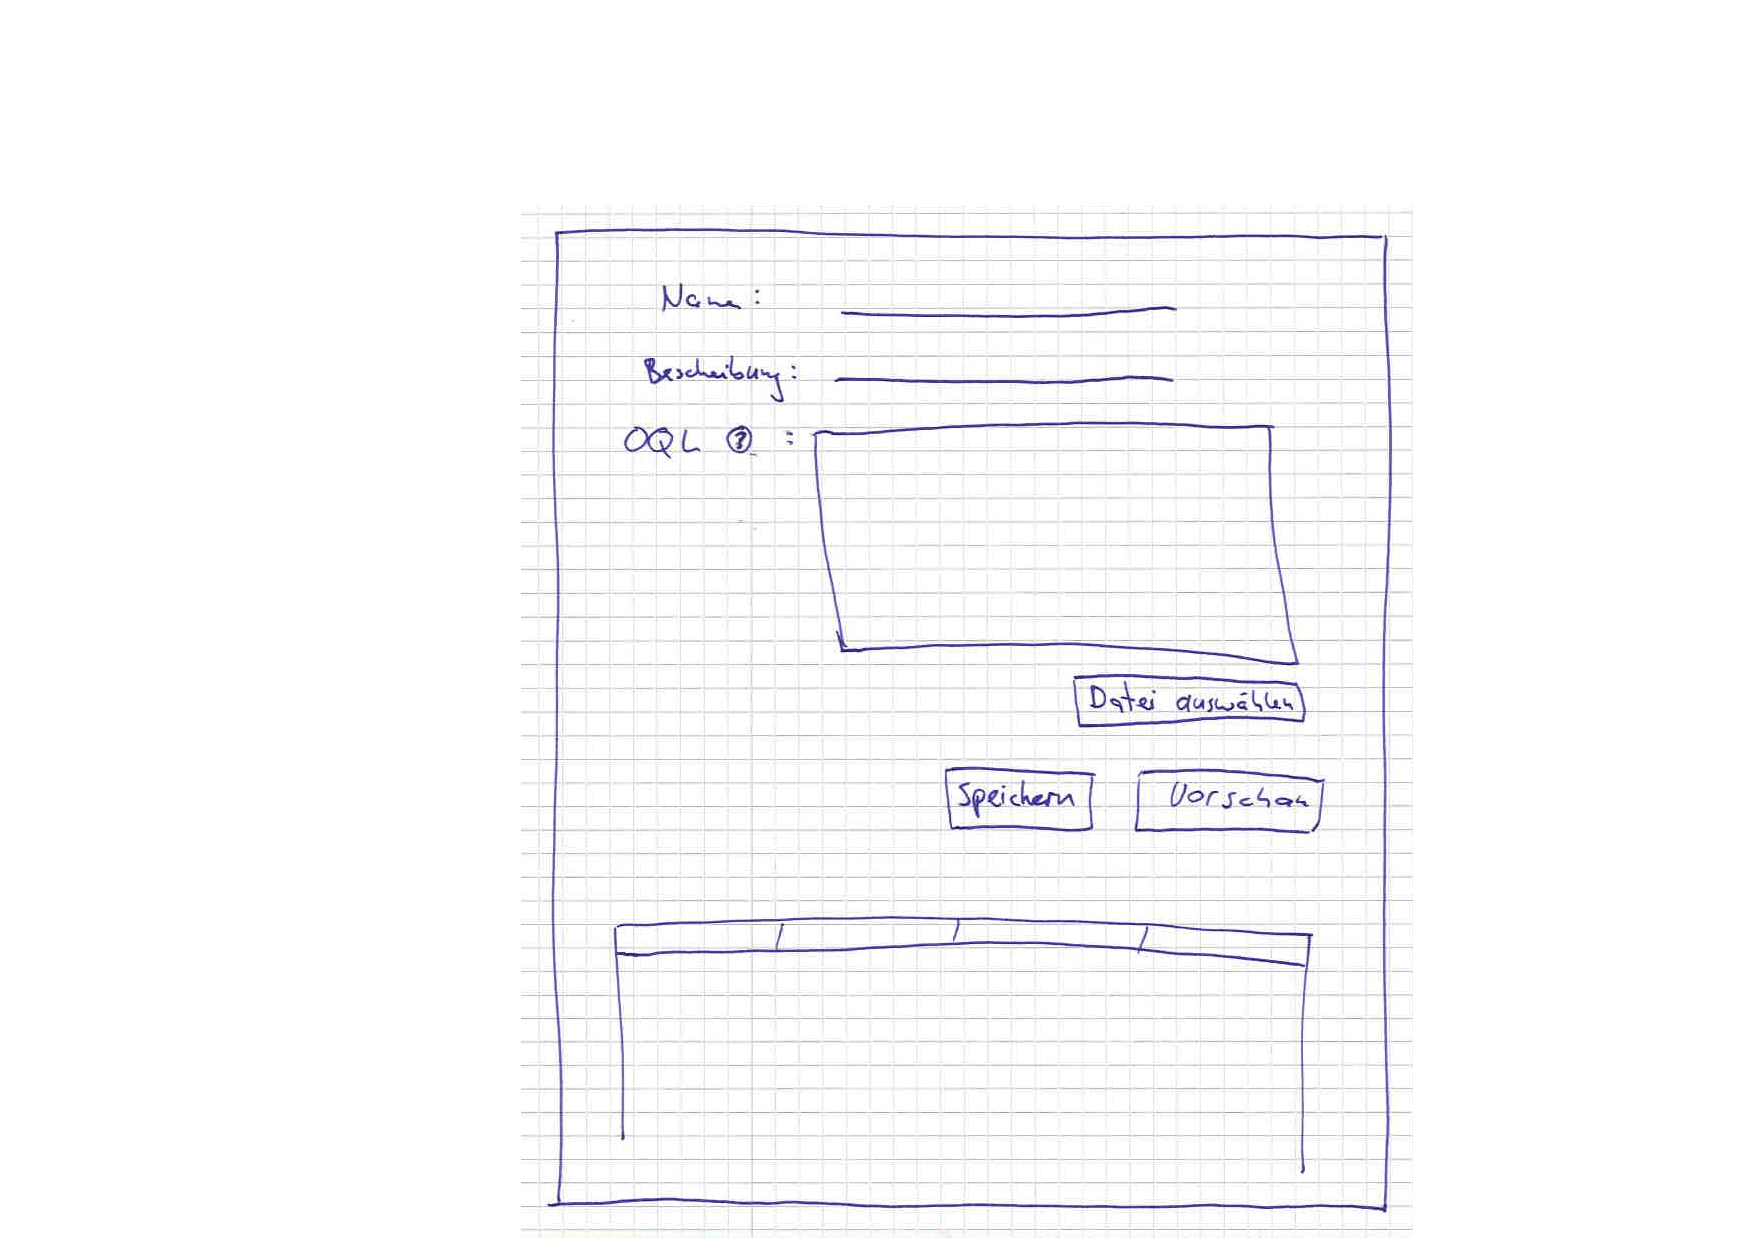
\includegraphics[width=0.8\linewidth]{fig/mockup_hcdi}
    \caption{Frühes Mockup ``Transformation erstellen''}
    \label{fig:pd:mockup-upload}
\end{figure}
Bevor uns klar wurde, dass eine neue Transformation einen Assistenten braucht, haben wir uns diesen Menupunkt wie in \cref{fig:pd:mockup-upload} vorgestellt. Später konnten wir uns vorstellen, einen grafischen Assistenten - ähnlich wie bei Yahoo Pipes (eingestellt) - zu implementieren. Aussehen können hätte dies wie in \cref{fig:pd:connectors} gezeigt.
\begin{figure}[H]
    \centering
    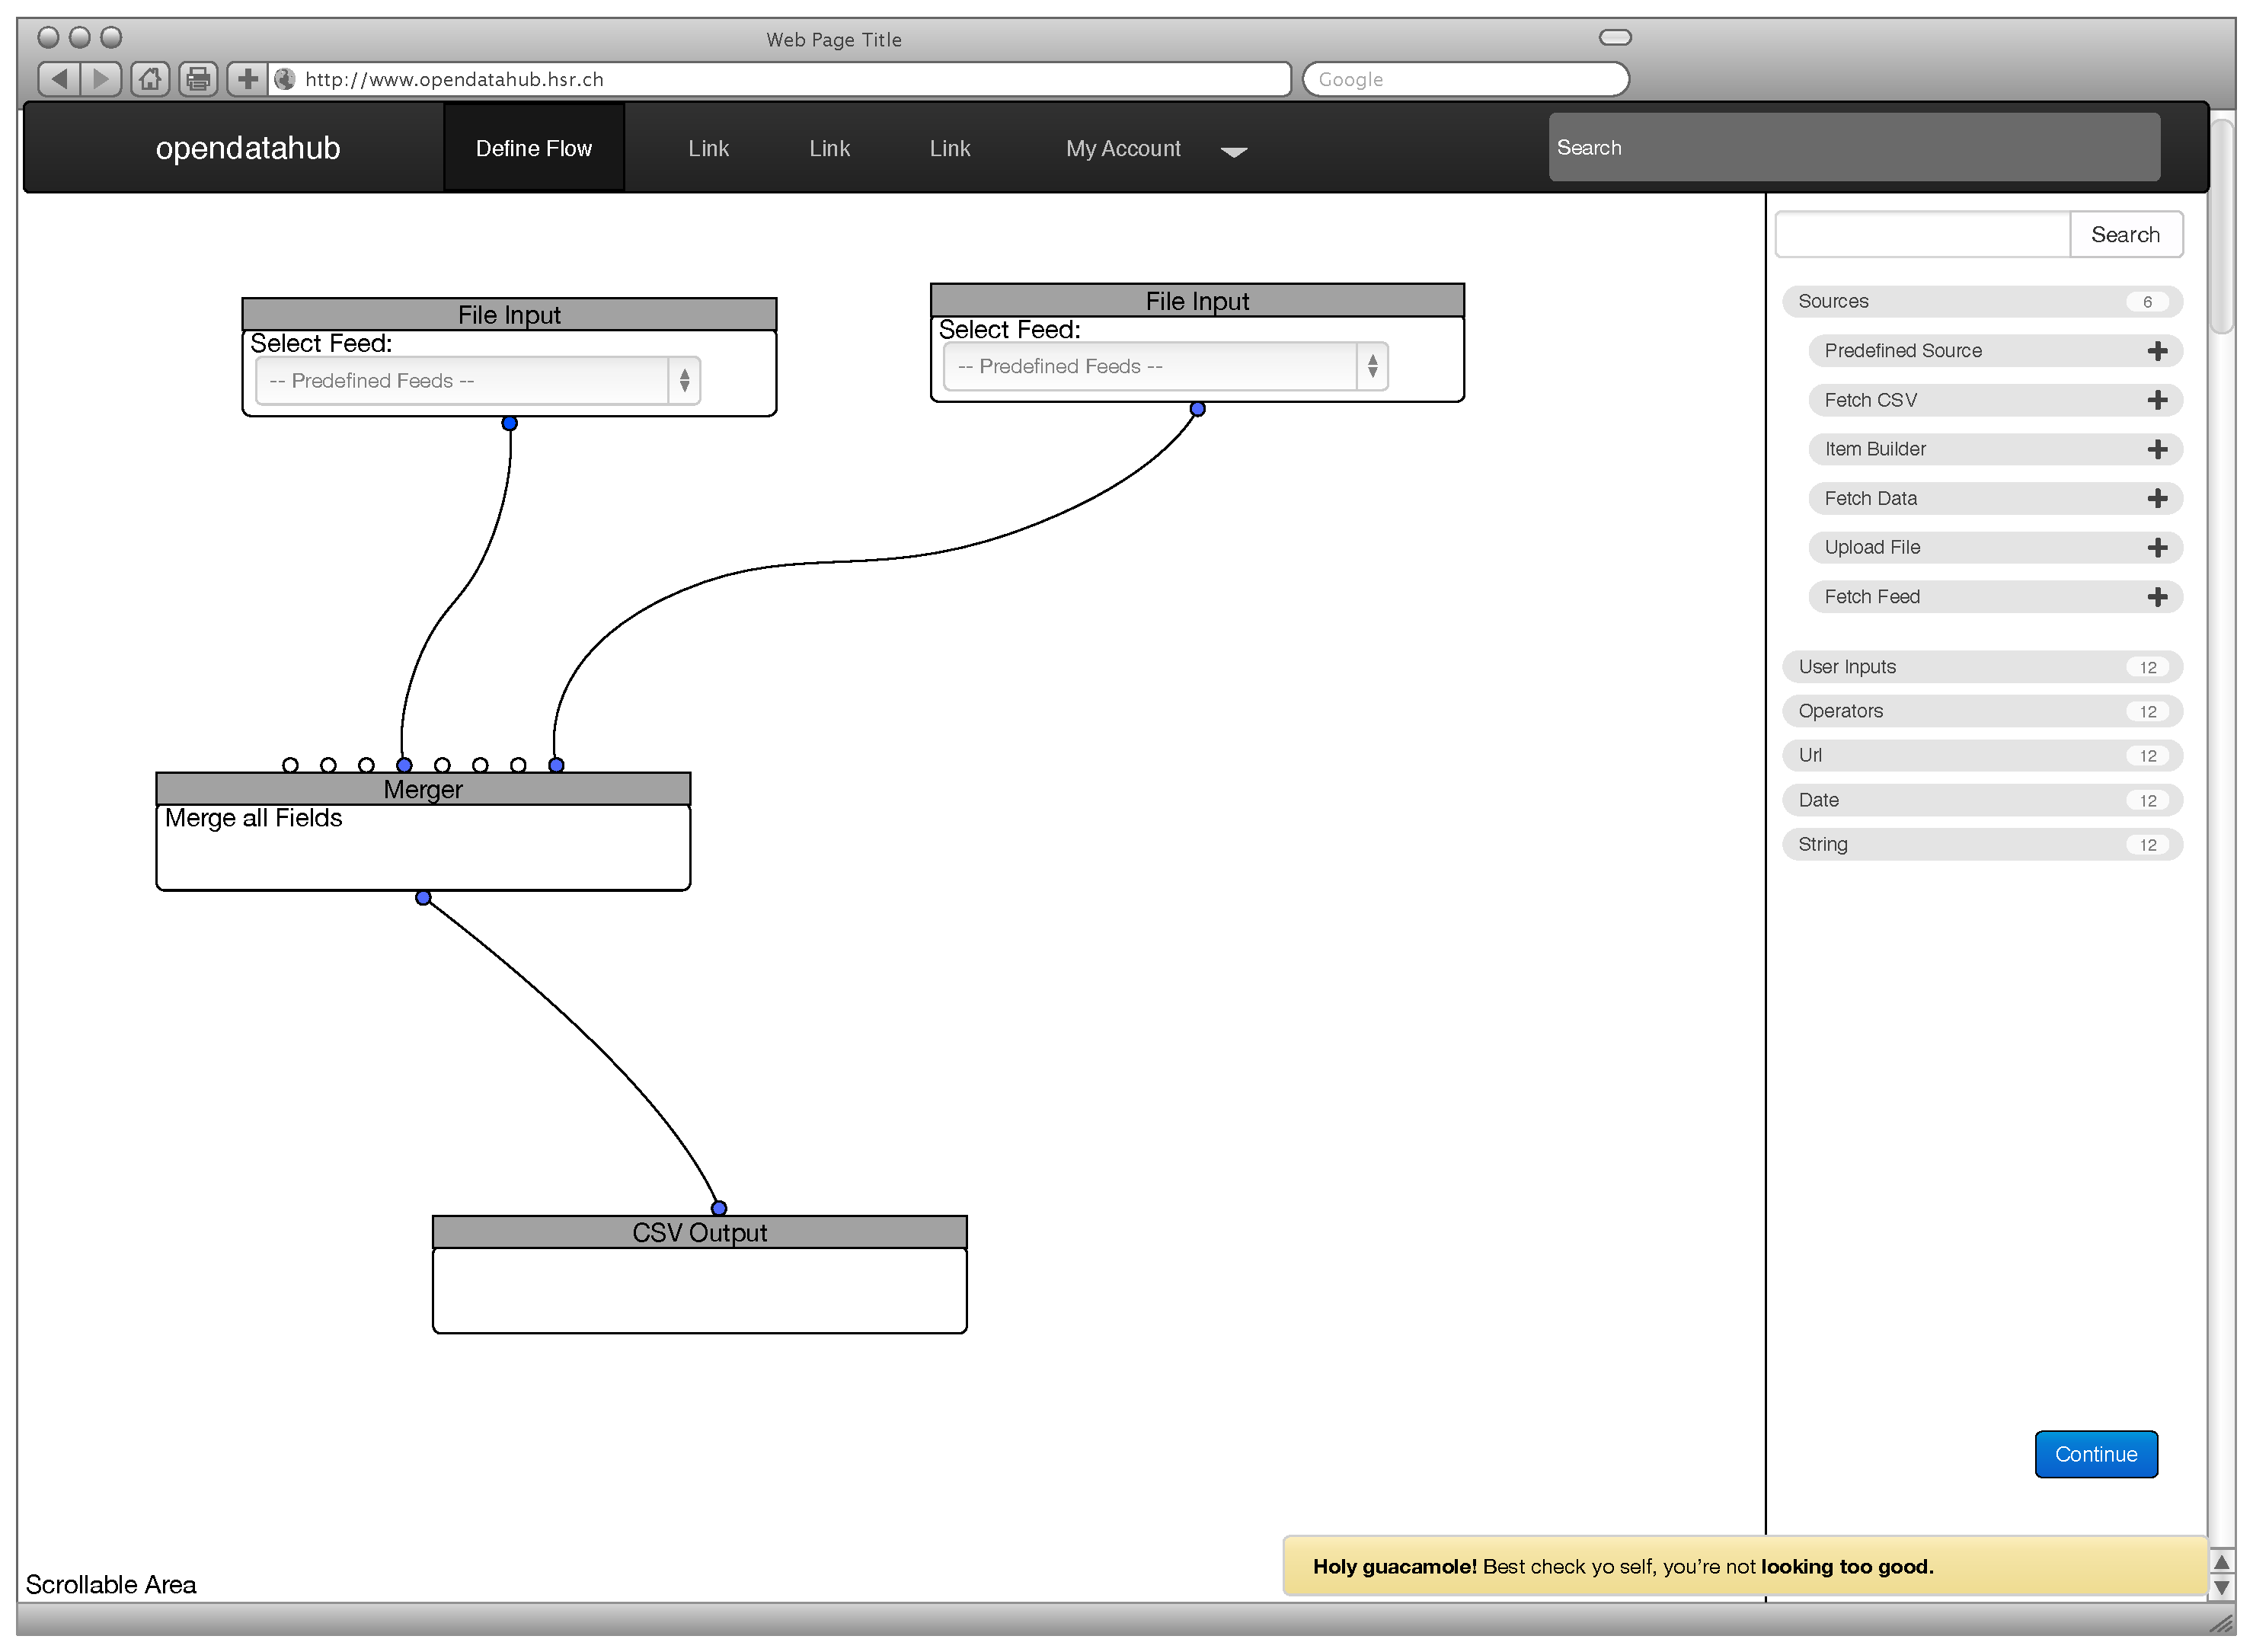
\includegraphics[width=0.8\linewidth]{fig/Wireframes-Connectors}
    \caption{Frühe Idee Transformation mit ``Pipes'' erstellen. (Verworfen)}
    \label{fig:pd:connectors}
\end{figure}
Das Upload-Formular haben wir ziemlich so implementiert, wie wir uns das in \cref{fig:pd:wireframe-upload} vorgestellt haben.
\begin{figure}[H]
    \centering
    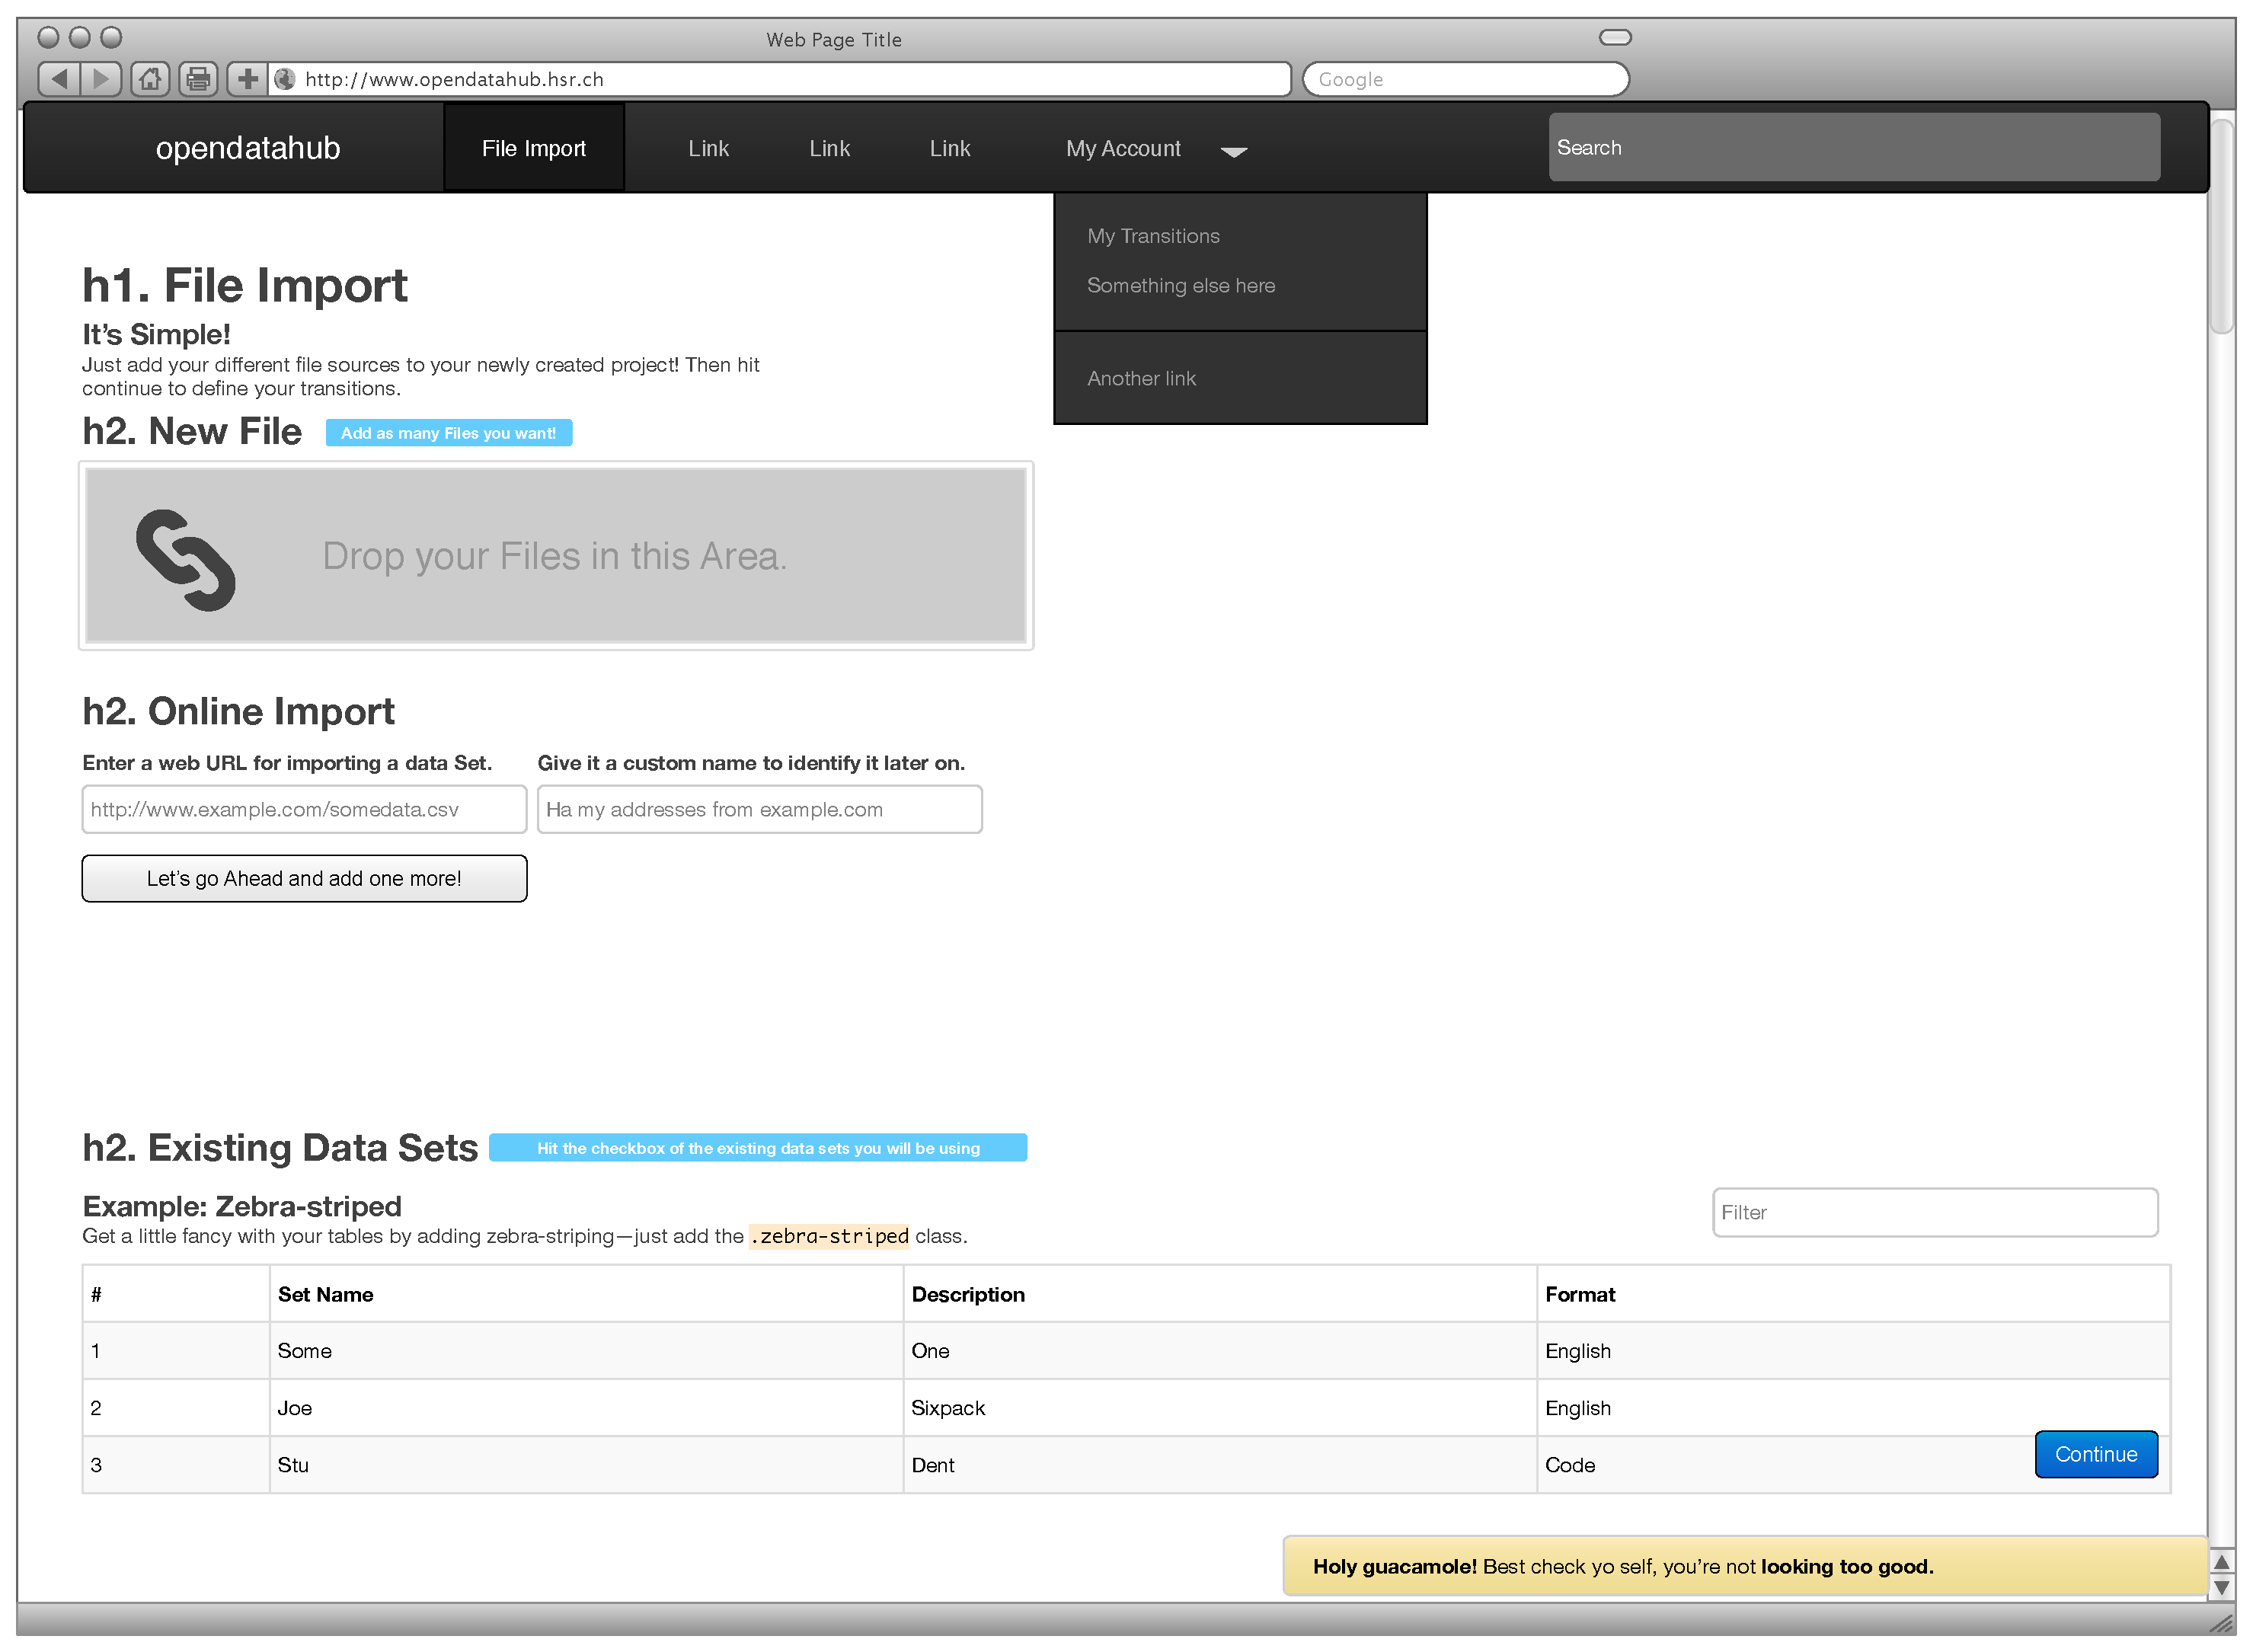
\includegraphics[width=0.8\linewidth]{fig/Wireframes-Upload}
    \caption{Frühes Mockup für Upload Formular}
    \label{fig:pd:wireframe-upload}
\end{figure}

\section{Benutzer-Authentifizierung}
In diesem Kapitel werden verscheidene Methoden der Authentifizierung beleuchtet.
\subsection{Herkömmliche Registrierung per E-Mail}
Die herkömmliche Registrierung bietet den Vorteil, dass sie keine Abhängigkeiten zu Dritt-Providern erfordert. So kann sich jeder Benutzer mit einer gültigen E-Mail Adresse einloggen. Ein Nachteil dieser Methode kann sein, dass Dummy-Adressen verwendet werden können und so ein registrierter Benutzer nicht wirklich Authentifiziert ist. Nachteilig ist, dass der Benutzer nicht verifiziert ist. Benutzer müssen ein Passwort speziell für diesen Service erstellen um den persönlichen Sicherheitsansprüchen zu genügen.
\subsection{oAuth2}
oAuth2 hat einen anderen Ansatz. Sociale Netzwerke bieten sich an, um mit den Login-Daten des bereits bestehenden Accounts in einem solchen ein Account bei opendatahub zu erstellen. So ist der Benutzer der sich registriert bereits authentifizert und es kann davon ausgegangen werden, dass es sich wirklich um diesen handelt. Die häufigkeit von``Fake-Profilen'' wird dadurch reduziert. Auch muss der Benutzer kein weiteres Passwort wissen.
\subsection{Fazit}
Obwohl sich diese Methoden verbinden liessen, setzen wir einzig und alleine auf die oAuth Methode.
\begin{decision}{Benutzer-Authentifizierung}
Aufgrund der Entscheidung das Benutzer-Handling einfach zu halten, haben wir uns dazu entschieden nur auf die Methoden zur Authentifizierung per GitHub und Facebook zu basieren.
\end{decision}

\section{Session-Authentifizierung}
\subsection{Cookie-Based-Authentication}
Bei der Cookie-Based-Authentifizierung wird eine Session-ID auf der Seite des Clients in einem Server-Side Cookie gespeichert. Dieses wird mit jedem Request an den Server übermittelt. So kann der Server davon ausgehen, dass es sich beim Client um den Inhaber der Session ID handelt.

\subsection{Token-Based-Authentication}
Ein neuerer Ansatz, ist es, einen Signierten Token im Header jedes Requests der zum Server geht mitzusenden. Vorteile dieser Variante sind bestechend:
\begin{description}
  \item[Cross-Domain / CORS]
  Cookies und CORS spielen nicht so sauber zwischen mehreren Domains. Ein Token basierter Ansatz erlaubt es AJAX Aufrufe an jeden Server mit jeder Domain zu veranlassen, weil die Informationen im HTTP Header liegen.
  \item[Stateless (Server-Side-Scalability)]Es wird kein Session-Store benötigt. Der Token enthält alle Benutzerinformationen der Rest des `States' liegt im Local Storage auf der Client-Side.
  \item[Decoupling] Man ist nicht an ein Authentifizierungs-Schema gebunden. Der Token kann überall generiert werden, sprich die API kann von überall her aufgerufen werden.
  \item[Mobile-Ready]Cookies sind in nativen mobilen Apps böse.
  \item[CSRF]Cross-Site Requests stellen kein Problem dar. Es gibt kein Authentication Cookie, das wiederverwendet werden könnte.
  \item[Standard]Es gibt bereits einen Standard. (\gls{JWT})
\end{description}
\begin{figure}[H]
    \centering
    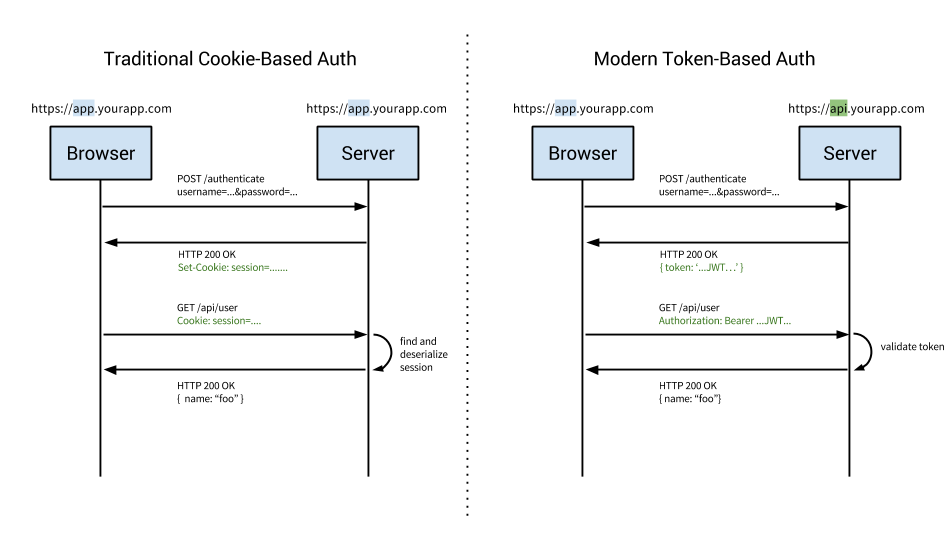
\includegraphics[width=\linewidth]{fig/cookie-token-auth}
    \caption{Cookie vs. Token Auth}
    \label{fig:pd:cookie-token-auth}
\end{figure}
\subsection{Fazit}
\begin{decision}{Session-Authentifizierung}
Da wir die API vom Frontend so klar wie möglich trennen wollen, setzen wir auf die modernere Variante mittels \acs{JWT}. So könnte die API auch auf einer anderen Domain wie das Frontend liegen.
\end{decision}
